フロアマップ情報を用いた初期方向補正ではマップの存在可能な点の分布によっては正しく機能しない場合がある.
別の方法としてBLEビーコンの基地局の位置情報を用いた初期方向補正を行う関数を提供する.
関数をListing\ref{lst:rotate-trajectory-using-ble}に示す.
この関数では加速度DF,角度DF,BLEビーコンの受信電波DF, BLEビーコンの基地局DFを受け取る.
BLEビーコンの受信電波DFとBLEビーコンの基地局DFのカラム名とデータ型を表6,表7に示す.
戻り値は時間経過に伴う2次元座標のDFと角度のDFを返す.
一定の強いRSSIの電波を受信した際の時間情報を元に時間的に近い推定軌跡の座標を取得する.
図\ref{fig:ble-merge}に示した図は時間的に近い推定軌跡の座標を時間経過に応じた色で表しており
青色の座標が配置されたBLEビーコンの座標を表している.

推定した軌跡の受信したBLEビーコンの基地局の座標との距離を計算する.
この総和が最小となるような回転角度をグリッドサーチで探し最適な角度に補正を行う.
BLEビーコンの基地局の座標との距離を計算する.

\begin{lstlisting}[caption={BLEビーコンの基地局の位置情報を使用した初期方向補正}, label=lst:rotate-trajectory-using-ble]
def rotate_trajectory_to_optimal
		_alignment_using_ble(
    acc_df: pd.DataFrame,
    angle_df: pd.DataFrame,
    ble_scans_df: pd.DataFrame,
    ble_position_df: pd.DataFrame,
    *,
    ground_truth_first_point: dict[Axis2D, float] | None = None,
) -> tuple[pd.DataFrame, pd.DataFrame]:
\end{lstlisting}


\begin{figure}[ht]
	\centering
	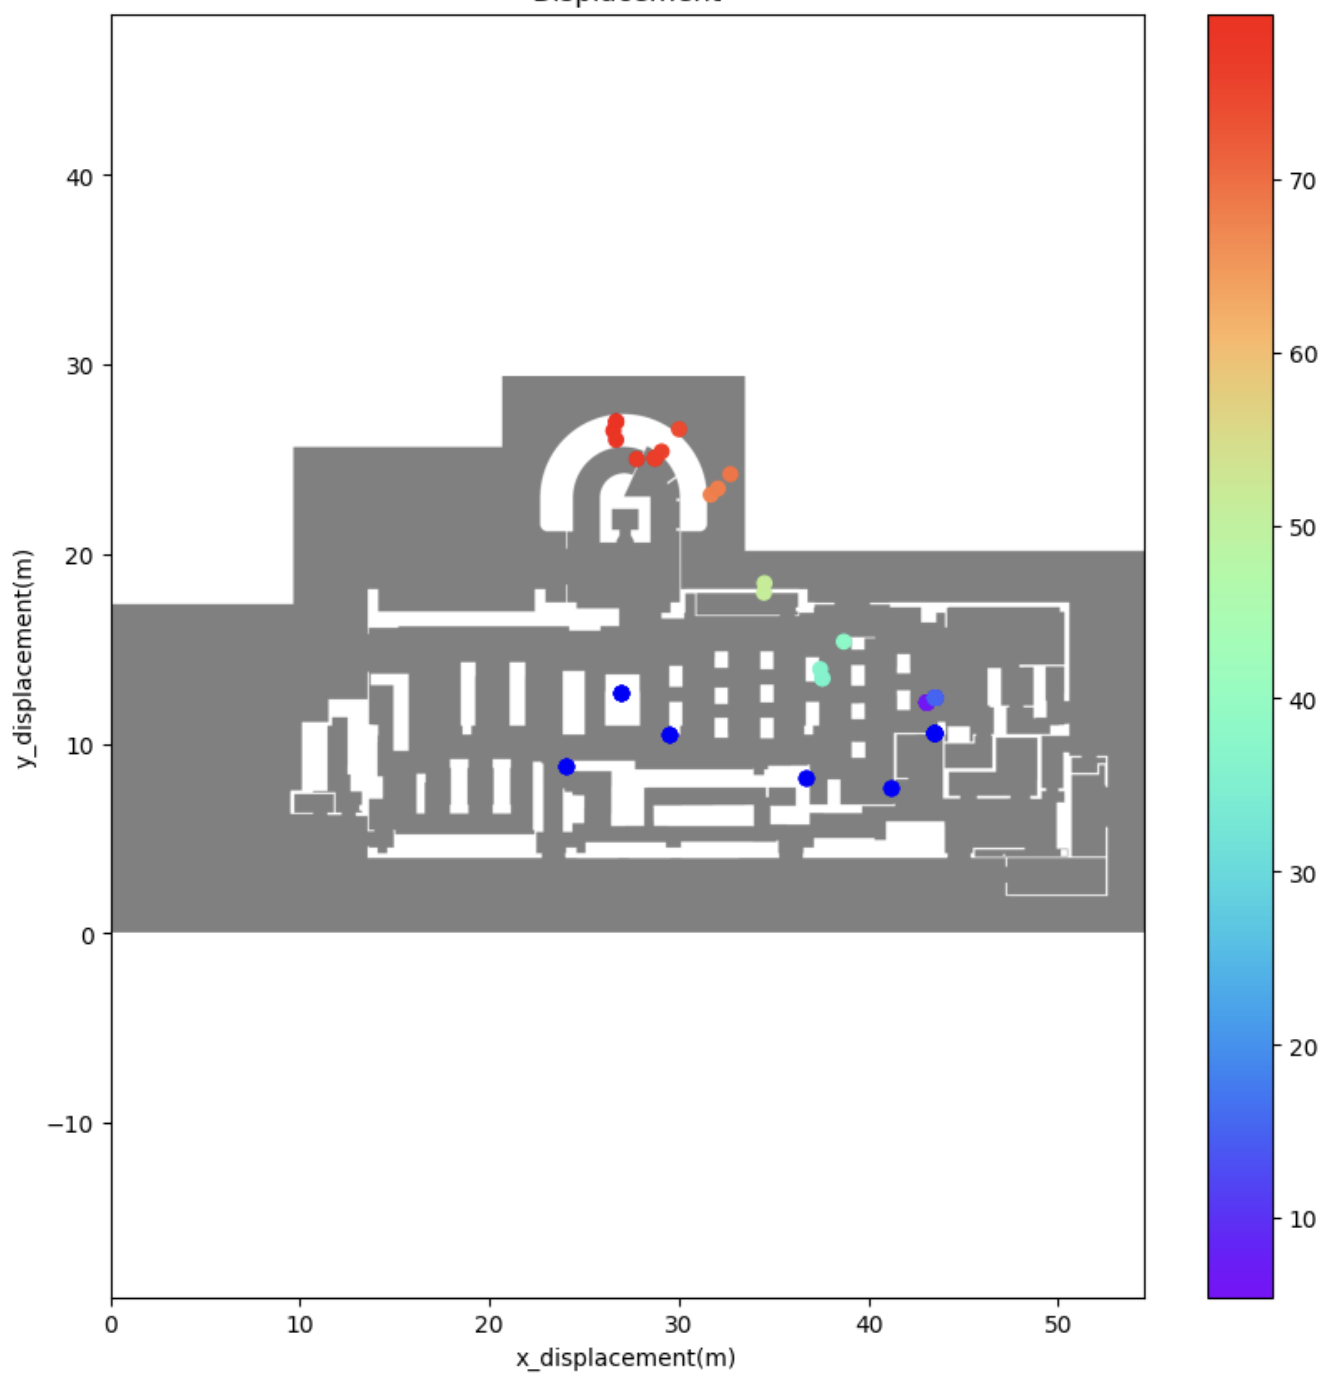
\includegraphics[width=80mm]{image/ble-merge.jpg}
	\caption{強いビーコン電波を受信した際の\\時間的に近い軌跡の座標}    \label{fig:ble-merge}
\end{figure}

\begin{table}[ht]
	\centering
	\begin{tabular}{lll}
		\toprule
		カラム名      & 単位    & データ型  \\
		\midrule
		ts        & s (秒) & float \\
		bdaddress & なし    & str   \\
		rssi      & dBm   & int   \\
		\bottomrule
	\end{tabular}
	\caption{BLEビーコン受信電波 DF}
\end{table}

\begin{table}[ht]
	\centering
	\begin{tabular}{lll}
		\toprule
		カラム名        & 単位 & データ型  \\
		\midrule
		bdaddress   & なし & str   \\
		x           & m  & float \\
		y           & m  & float \\
		floor\_name & なし & str   \\
		\bottomrule
	\end{tabular}
	\caption{BLEビーコン基地局 DF}
\end{table}
